%%%%%%%%%%%%%%%%%%%%%%%%%%%%%%%%%%%%%%%%%%%%%%%%%%%%%%%%%%%

%% document class
\documentclass[a4paper,11pt,oneside]{book}

%% packages
%% packages

\usepackage{blindtext} % needed for creating dummy text passages
%\usepackage{ngerman} % needed for German default language
\usepackage{amsmath} % needed for command eqref
\usepackage{amssymb} % needed for math fonts
\usepackage[
	colorlinks=true
	,breaklinks
	%,ngerman
	]{hyperref} % needed for creating hyperlinks in the document, the option colorlinks=true gets rid of the awful boxes, breaklinks breaks lonkg links (list of figures), and ngerman sets everything for german as default hyperlinks language
\usepackage[hyphenbreaks]{breakurl} % ben�tigt f�r das Brechen von URLs in Literaturreferenzen, hyphenbreaks auch bei links, die �ber eine Seite gehen (mit hyphenation).
\usepackage{xcolor}
\definecolor{c1}{rgb}{0,0,1} % blue
\definecolor{c2}{rgb}{0,0.3,0.9} % light blue
\definecolor{c3}{rgb}{0.3,0,0.9} % red blue
\hypersetup{
    linkcolor={c1}, % internal links
    citecolor={c2}, % citations
    urlcolor={c3} % external links/urls
}
%\usepackage{cite} % needed for cite
\usepackage[round,authoryear]{natbib} % needed for cite and abbrvnat bibliography style
\usepackage[nottoc]{tocbibind} % needed for displaying bibliography and other in the table of contents
\usepackage{graphicx} % needed for \includegraphics 
\usepackage{longtable} % needed for long tables over pages
\usepackage{bigstrut} % needed for the command \bigstrut
\usepackage{enumerate} % needed for some options in enumerate
\usepackage{array}
\usepackage{textgreek}
\usepackage{todonotes} % needed for todos
\usepackage{makeidx} % needed for creating an index
\makeindex
\usepackage{placeins}
\usepackage [english]{babel}
\usepackage [autostyle, english = american]{csquotes}
\MakeOuterQuote{"}
\usepackage{multirow}
\usepackage{dcolumn}
\usepackage{array}
\usepackage{makecell}

%% page settings
%% page settings

\usepackage[top=2cm, bottom=1.8cm,left=2.5cm,right=2.5cm]{geometry} % needed for page border settings
\parindent=0cm % for space of first line of new text block
\sloppy % for writing with hyphenless justification (tries to)
\hyphenation{} % use hyphenation of tolerance parameters, http://www.jr-x.de/publikationen/latex/tipps/zeilenumbruch.html
\hyphenpenalty=10000
\exhyphenpenalty=10000
\usepackage{fancyhdr} % needed for head and foot options

%% own commands
%\newcommand{\tbi}[1]{\textbf{\textit{#1}}}
%% my macros

%% Text fomats
\newcommand{\tbi}[1]{\textbf{\textit{#1}}}

%% Math fonts
\newcommand{\bbA}{\mathbb{A}}
\newcommand{\bbB}{\mathbb{B}}
\newcommand{\bbC}{\mathbb{C}}
\newcommand{\bbD}{\mathbb{D}}
\newcommand{\bbE}{\mathbb{E}}
\newcommand{\bbF}{\mathbb{F}}
\newcommand{\bbG}{\mathbb{G}}
\newcommand{\bbH}{\mathbb{H}}
\newcommand{\bbI}{\mathbb{I}}
\newcommand{\bbJ}{\mathbb{J}}
\newcommand{\bbK}{\mathbb{K}}
\newcommand{\bbL}{\mathbb{L}}
\newcommand{\bbM}{\mathbb{M}}
\newcommand{\bbN}{\mathbb{N}}
\newcommand{\bbO}{\mathbb{O}}
\newcommand{\bbP}{\mathbb{P}}
\newcommand{\bbQ}{\mathbb{Q}}
\newcommand{\bbR}{\mathbb{R}}
\newcommand{\bbS}{\mathbb{S}}
\newcommand{\bbT}{\mathbb{T}}
\newcommand{\bbU}{\mathbb{U}}
\newcommand{\bbV}{\mathbb{V}}
\newcommand{\bbW}{\mathbb{W}}
\newcommand{\bbX}{\mathbb{X}}
\newcommand{\bbY}{\mathbb{Y}}
\newcommand{\bbZ}{\mathbb{Z}}
\newcommand{\imp}[1]{\underline{\textit{#1}}}

%%%%%%%%%%%%%%%%%%%%%%%%%%%%%%%%%%%%%%%%%%%%%%%%%%%%%%%%%%%

\begin{document}

%%%%%%%%%%%%%%%%%%%%%%%%%%%%%%%%%%%%%%%%%%%%%%%%%%%%%%%%%%%
%%%%%%%%%%%%%%%%%%%%%%%%%%%%%%%%%%%%%%%%%%%%%%%%%%%%%%%%%%%
%%%%%%%%%%%%%%%%%%%%%%%%%%%%%%%%%%%%%%%%%%%%%%%%%%%%%%%%%%%

%\pagestyle{empty}
%\title{Basic elements for writing a book/thesis using \LaTeX}
%\author{Mauricio Lobos}
%\date{}
%\maketitle
%%%%%%%%%%%%%%%%%%%%%%%%%%%%%%%%%%%%%%%%%
% University Assignment Title Page 
% LaTeX Template
% Version 1.0 (27/12/12)
%
% This template has been downloaded from:
% http://www.LaTeXTemplates.com
%
% Original author:
% WikiBooks (http://en.wikibooks.org/wiki/LaTeX/Title_Creation)
%
% License:
% CC BY-NC-SA 3.0 (http://creativecommons.org/licenses/by-nc-sa/3.0/)
% 
% Instructions for using this template:
% This title page is capable of being compiled as is. This is not useful for 
% including it in another document. To do this, you have two options: 
%
% 1) Copy/paste everything between \begin{document} and \end{document} 
% starting at \begin{} and paste this into another LaTeX file where you 
% want your title page.
% OR
% 2) Remove everything outside the \begin{titlepage} and \end{titlepage} and 
% move this file to the same directory as the LaTeX file you wish to add it to. 
% Then add %%%%%%%%%%%%%%%%%%%%%%%%%%%%%%%%%%%%%%%%%
% University Assignment Title Page 
% LaTeX Template
% Version 1.0 (27/12/12)
%
% This template has been downloaded from:
% http://www.LaTeXTemplates.com
%
% Original author:
% WikiBooks (http://en.wikibooks.org/wiki/LaTeX/Title_Creation)
%
% License:
% CC BY-NC-SA 3.0 (http://creativecommons.org/licenses/by-nc-sa/3.0/)
% 
% Instructions for using this template:
% This title page is capable of being compiled as is. This is not useful for 
% including it in another document. To do this, you have two options: 
%
% 1) Copy/paste everything between \begin{document} and \end{document} 
% starting at \begin{} and paste this into another LaTeX file where you 
% want your title page.
% OR
% 2) Remove everything outside the \begin{titlepage} and \end{titlepage} and 
% move this file to the same directory as the LaTeX file you wish to add it to. 
% Then add %%%%%%%%%%%%%%%%%%%%%%%%%%%%%%%%%%%%%%%%%
% University Assignment Title Page 
% LaTeX Template
% Version 1.0 (27/12/12)
%
% This template has been downloaded from:
% http://www.LaTeXTemplates.com
%
% Original author:
% WikiBooks (http://en.wikibooks.org/wiki/LaTeX/Title_Creation)
%
% License:
% CC BY-NC-SA 3.0 (http://creativecommons.org/licenses/by-nc-sa/3.0/)
% 
% Instructions for using this template:
% This title page is capable of being compiled as is. This is not useful for 
% including it in another document. To do this, you have two options: 
%
% 1) Copy/paste everything between \begin{document} and \end{document} 
% starting at \begin{} and paste this into another LaTeX file where you 
% want your title page.
% OR
% 2) Remove everything outside the \begin{titlepage} and \end{titlepage} and 
% move this file to the same directory as the LaTeX file you wish to add it to. 
% Then add \input{./title_page_1.tex} to your LaTeX file where you want your
% title page.
%
%%%%%%%%%%%%%%%%%%%%%%%%%%%%%%%%%%%%%%%%%

%----------------------------------------------------------------------------------------
%	PACKAGES AND OTHER DOCUMENT CONFIGURATIONS
%----------------------------------------------------------------------------------------

%\documentclass[12pt]{article}
%
%\begin{document}

\begin{titlepage}
	

\newcommand{\HRule}{\rule{\linewidth}{0.5mm}} % Defines a new command for the horizontal lines, change thickness here

\center % Center everything on the page
 
%----------------------------------------------------------------------------------------
%	HEADING SECTIONS
%----------------------------------------------------------------------------------------
\begin{minipage}[b]{0.4\textwidth}
	%\begin{flushleft} \large
	\begin{center}
		
\includegraphics[width=0.5\textwidth]{figures/download}\\[1cm] % Include a department/university logo - this will require the graphicx package
		%\end{flushleft}
	\end{center}
\end{minipage}
\vspace{1.5cm}



\textsc{\LARGE Department of Financial Mathematics}\\[1.5cm] % Name of your university/college
\textsc{\Large }\\[0.5cm] % Major heading such as course name
\textsc{\large }\\[0.5cm] % Minor heading such as course title

%----------------------------------------------------------------------------------------
%	TITLE SECTION
%----------------------------------------------------------------------------------------

\HRule \\[0.5cm]
{ \huge \bfseries Comparison of Forecasting Models for Value at Risk}\\[0.1cm] % Title of your document
\HRule \\[1.5cm]
\vspace{2.5cm}
 
%----------------------------------------------------------------------------------------
%	AUTHOR SECTION
%----------------------------------------------------------------------------------------


\begin{minipage}{0.4\textwidth}
\begin{flushleft} \large
\emph{Author:}\\
Hafees Adebayo \textsc{Yusuff} % Your name
\end{flushleft}
\end{minipage}
~
\begin{minipage}{0.4\textwidth}
\begin{flushleft} \large
\emph{Supervisor:} \\
Prof. Ralf \textsc{Korn} % Supervisor's Name
\end{flushleft}
\end{minipage}\\[4cm]

% If you don't want a supervisor, uncomment the two lines below and remove the section above
%\Large \emph{Author:}\\
%John \textsc{Smith}\\[3cm] % Your name

%----------------------------------------------------------------------------------------

%	DATE SECTION
%----------------------------------------------------------------------------------------

{\large \today}\\[3cm] % Date, change the \today to a set date if you want to be precise
\vspace{2.5cm}


A thesis submitted in fulfilment of the requirements for the degree of
Master of Science

%----------------------------------------------------------------------------------------
%	LOGO SECTION
%----------------------------------------------------------------------------------------

%~
%\begin{minipage}[b]{0.4\textwidth}
%\begin{flushleft} \large
%
\includegraphics[width=0.5\textwidth]{figures/download (1)}
%\end{flushleft}
%\end{minipage}

%----------------------------------------------------------------------------------------

\vfill % Fill the rest of the page with whitespace
\end{titlepage}



\thispagestyle{empty}

\newpage\null\thispagestyle{empty}\newpage


\begin{titlepage}
	\textbf{\LARGE Declaration of Authorship}\newline\newline
	

		
		I, Hafees Adebayo YUSUFF, hereby declare the following thesis titled "Comparison of forecasting models for value at risk" to be my own work and I confirm that:
			\begin{itemize}
		\item[$\bullet$] The thesis I am submitting is entirely my own work except where otherwise indicated.
		
		\item[$\bullet$] It has not been submitted, either partially or in full, for a qualification at this or any other University.
	
	\item[$\bullet$] I have clearly signalled the presence of all material I have quoted from other sources,
	including any diagrams, charts, tables or graphs.
	
	\item[$\bullet$] I have acknowledged appropriately any assistance I have received.
	
	\end{itemize}
	
	\vspace*{4em}\noindent
	\hfill%
	\begin{tabular}[t]{c}
		\rule{10em}{0.4pt}\\ Signature
	\end{tabular}%
	\hfill%
	\begin{tabular}[t]{c}
		\rule{10em}{0.4pt}\\ Date
	\end{tabular}%
	\hfill\strut


\end{titlepage}
 to your LaTeX file where you want your
% title page.
%
%%%%%%%%%%%%%%%%%%%%%%%%%%%%%%%%%%%%%%%%%

%----------------------------------------------------------------------------------------
%	PACKAGES AND OTHER DOCUMENT CONFIGURATIONS
%----------------------------------------------------------------------------------------

%\documentclass[12pt]{article}
%
%\begin{document}

\begin{titlepage}
	

\newcommand{\HRule}{\rule{\linewidth}{0.5mm}} % Defines a new command for the horizontal lines, change thickness here

\center % Center everything on the page
 
%----------------------------------------------------------------------------------------
%	HEADING SECTIONS
%----------------------------------------------------------------------------------------
\begin{minipage}[b]{0.4\textwidth}
	%\begin{flushleft} \large
	\begin{center}
		
\includegraphics[width=0.5\textwidth]{figures/download}\\[1cm] % Include a department/university logo - this will require the graphicx package
		%\end{flushleft}
	\end{center}
\end{minipage}
\vspace{1.5cm}



\textsc{\LARGE Department of Financial Mathematics}\\[1.5cm] % Name of your university/college
\textsc{\Large }\\[0.5cm] % Major heading such as course name
\textsc{\large }\\[0.5cm] % Minor heading such as course title

%----------------------------------------------------------------------------------------
%	TITLE SECTION
%----------------------------------------------------------------------------------------

\HRule \\[0.5cm]
{ \huge \bfseries Comparison of Forecasting Models for Value at Risk}\\[0.1cm] % Title of your document
\HRule \\[1.5cm]
\vspace{2.5cm}
 
%----------------------------------------------------------------------------------------
%	AUTHOR SECTION
%----------------------------------------------------------------------------------------


\begin{minipage}{0.4\textwidth}
\begin{flushleft} \large
\emph{Author:}\\
Hafees Adebayo \textsc{Yusuff} % Your name
\end{flushleft}
\end{minipage}
~
\begin{minipage}{0.4\textwidth}
\begin{flushleft} \large
\emph{Supervisor:} \\
Prof. Ralf \textsc{Korn} % Supervisor's Name
\end{flushleft}
\end{minipage}\\[4cm]

% If you don't want a supervisor, uncomment the two lines below and remove the section above
%\Large \emph{Author:}\\
%John \textsc{Smith}\\[3cm] % Your name

%----------------------------------------------------------------------------------------

%	DATE SECTION
%----------------------------------------------------------------------------------------

{\large \today}\\[3cm] % Date, change the \today to a set date if you want to be precise
\vspace{2.5cm}


A thesis submitted in fulfilment of the requirements for the degree of
Master of Science

%----------------------------------------------------------------------------------------
%	LOGO SECTION
%----------------------------------------------------------------------------------------

%~
%\begin{minipage}[b]{0.4\textwidth}
%\begin{flushleft} \large
%
\includegraphics[width=0.5\textwidth]{figures/download (1)}
%\end{flushleft}
%\end{minipage}

%----------------------------------------------------------------------------------------

\vfill % Fill the rest of the page with whitespace
\end{titlepage}



\thispagestyle{empty}

\newpage\null\thispagestyle{empty}\newpage


\begin{titlepage}
	\textbf{\LARGE Declaration of Authorship}\newline\newline
	

		
		I, Hafees Adebayo YUSUFF, hereby declare the following thesis titled "Comparison of forecasting models for value at risk" to be my own work and I confirm that:
			\begin{itemize}
		\item[$\bullet$] The thesis I am submitting is entirely my own work except where otherwise indicated.
		
		\item[$\bullet$] It has not been submitted, either partially or in full, for a qualification at this or any other University.
	
	\item[$\bullet$] I have clearly signalled the presence of all material I have quoted from other sources,
	including any diagrams, charts, tables or graphs.
	
	\item[$\bullet$] I have acknowledged appropriately any assistance I have received.
	
	\end{itemize}
	
	\vspace*{4em}\noindent
	\hfill%
	\begin{tabular}[t]{c}
		\rule{10em}{0.4pt}\\ Signature
	\end{tabular}%
	\hfill%
	\begin{tabular}[t]{c}
		\rule{10em}{0.4pt}\\ Date
	\end{tabular}%
	\hfill\strut


\end{titlepage}
 to your LaTeX file where you want your
% title page.
%
%%%%%%%%%%%%%%%%%%%%%%%%%%%%%%%%%%%%%%%%%

%----------------------------------------------------------------------------------------
%	PACKAGES AND OTHER DOCUMENT CONFIGURATIONS
%----------------------------------------------------------------------------------------

%\documentclass[12pt]{article}
%
%\begin{document}

\begin{titlepage}
	

\newcommand{\HRule}{\rule{\linewidth}{0.5mm}} % Defines a new command for the horizontal lines, change thickness here

\center % Center everything on the page
 
%----------------------------------------------------------------------------------------
%	HEADING SECTIONS
%----------------------------------------------------------------------------------------
\begin{minipage}[b]{0.4\textwidth}
	%\begin{flushleft} \large
	\begin{center}
		
\includegraphics[width=0.5\textwidth]{figures/download}\\[1cm] % Include a department/university logo - this will require the graphicx package
		%\end{flushleft}
	\end{center}
\end{minipage}
\vspace{1.5cm}



\textsc{\LARGE Department of Financial Mathematics}\\[1.5cm] % Name of your university/college
\textsc{\Large }\\[0.5cm] % Major heading such as course name
\textsc{\large }\\[0.5cm] % Minor heading such as course title

%----------------------------------------------------------------------------------------
%	TITLE SECTION
%----------------------------------------------------------------------------------------

\HRule \\[0.5cm]
{ \huge \bfseries Comparison of Forecasting Models for Value at Risk}\\[0.1cm] % Title of your document
\HRule \\[1.5cm]
\vspace{2.5cm}
 
%----------------------------------------------------------------------------------------
%	AUTHOR SECTION
%----------------------------------------------------------------------------------------


\begin{minipage}{0.4\textwidth}
\begin{flushleft} \large
\emph{Author:}\\
Hafees Adebayo \textsc{Yusuff} % Your name
\end{flushleft}
\end{minipage}
~
\begin{minipage}{0.4\textwidth}
\begin{flushleft} \large
\emph{Supervisor:} \\
Prof. Ralf \textsc{Korn} % Supervisor's Name
\end{flushleft}
\end{minipage}\\[4cm]

% If you don't want a supervisor, uncomment the two lines below and remove the section above
%\Large \emph{Author:}\\
%John \textsc{Smith}\\[3cm] % Your name

%----------------------------------------------------------------------------------------

%	DATE SECTION
%----------------------------------------------------------------------------------------

{\large \today}\\[3cm] % Date, change the \today to a set date if you want to be precise
\vspace{2.5cm}


A thesis submitted in fulfilment of the requirements for the degree of
Master of Science

%----------------------------------------------------------------------------------------
%	LOGO SECTION
%----------------------------------------------------------------------------------------

%~
%\begin{minipage}[b]{0.4\textwidth}
%\begin{flushleft} \large
%
\includegraphics[width=0.5\textwidth]{figures/download (1)}
%\end{flushleft}
%\end{minipage}

%----------------------------------------------------------------------------------------

\vfill % Fill the rest of the page with whitespace
\end{titlepage}



\thispagestyle{empty}

\newpage\null\thispagestyle{empty}\newpage


\begin{titlepage}
	\textbf{\LARGE Declaration of Authorship}\newline\newline
	

		
		I, Hafees Adebayo YUSUFF, hereby declare the following thesis titled "Comparison of forecasting models for value at risk" to be my own work and I confirm that:
			\begin{itemize}
		\item[$\bullet$] The thesis I am submitting is entirely my own work except where otherwise indicated.
		
		\item[$\bullet$] It has not been submitted, either partially or in full, for a qualification at this or any other University.
	
	\item[$\bullet$] I have clearly signalled the presence of all material I have quoted from other sources,
	including any diagrams, charts, tables or graphs.
	
	\item[$\bullet$] I have acknowledged appropriately any assistance I have received.
	
	\end{itemize}
	
	\vspace*{4em}\noindent
	\hfill%
	\begin{tabular}[t]{c}
		\rule{10em}{0.4pt}\\ Signature
	\end{tabular}%
	\hfill%
	\begin{tabular}[t]{c}
		\rule{10em}{0.4pt}\\ Date
	\end{tabular}%
	\hfill\strut


\end{titlepage}
 % downloaded template

%\pagestyle{plain}
%\listoftodos
\tableofcontents

%%%%%%%%%%%%%%%%%%%%%%%%%%%%%%%%%%%%%%%%%%%%%%%%%%%%%%%%%%%
%%%%%%%%%%%%%%%%%%%%%%%%%%%%%%%%%%%%%%%%%%%%%%%%%%%%%%%%%%%
%%%%%%%%%%%%%%%%%%%%%%%%%%%%%%%%%%%%%%%%%%%%%%%%%%%%%%%%%%%

\chapter{Basics}

\pagestyle{fancy}
\fancyhf{}
\fancyhead[OC]{\leftmark}
\fancyhead[EC]{\rightmark}
%\renewcommand{\footrulewidth}{1pt}
\cfoot{\thepage}

%%%%%%%%%%%%%%%%%%%%%%%%%%%%%%%%%%%%%%%%%%%%%%%%%%%%%%%%%%%
%%%%%%%%%%%%%%%%%%%%%%%%%%%%%%%%%%%%%%%%%%%%%%%%%%%%%%%%%%%

\section{Section types}

The basic sections in a book are chapter, section, subsections and so on. These sections will appear in the \imp{tableofcontents} of the book.

%%%%%%%%%%%%%%%%%%%%%%%%%%%%%%%%%%%%%%%%%%%%%%%%%%%%%%%%%%%

\subsection{Example subsection}

This is just one example for a subsection.

%%%%%%%%%%%%%%%%%%%%%%%%%%%%%%%%%%%%%%%%%%%%%%%%%%%%%%%%%%%
%%%%%%%%%%%%%%%%%%%%%%%%%%%%%%%%%%%%%%%%%%%%%%%%%%%%%%%%%%%

\section{Basic page settings}

In order to show how the basic page settings are set up, we will use a long dummy text with the package \imp{blindtext}.

\blindtext[6]

\blindtext

\blindtext[7]

%%%%%%%%%%%%%%%%%%%%%%%%%%%%%%%%%%%%%%%%%%%%%%%%%%%%%%%%%%%
%%%%%%%%%%%%%%%%%%%%%%%%%%%%%%%%%%%%%%%%%%%%%%%%%%%%%%%%%%%

\section{Head and foot}

The head and foot of the document can be adapted using the packages \imp{fancyhdr}. The using the commands, e.g., \imp{pagestyle\{fancy\}}, \imp{l/c/rhead/foot} or with \imp{fancyhead/foot[EL,CO]} the respective parts can be edited as needed.

%%%%%%%%%%%%%%%%%%%%%%%%%%%%%%%%%%%%%%%%%%%%%%%%%%%%%%%%%%%
%%%%%%%%%%%%%%%%%%%%%%%%%%%%%%%%%%%%%%%%%%%%%%%%%%%%%%%%%%%

\section{New commands and input}

If some long commands for formatting or other utilities are used very often, e.g., \textbf{test}, \textit{test}, \textbf{\textit{test}}, then the definition of new personal commands is very useful. For this the command \imp{newcommand} is used before the document, e.g., \tbi{test}. Over time the collection of personal commands will grow, so for these it is better to create a separate file and copy this file to the current project folder. The file can be then loaded within the project with the command \imp{input} before the document.

%%%%%%%%%%%%%%%%%%%%%%%%%%%%%%%%%%%%%%%%%%%%%%%%%%%%%%%%%%%
%%%%%%%%%%%%%%%%%%%%%%%%%%%%%%%%%%%%%%%%%%%%%%%%%%%%%%%%%%%

\section{Language}

The default language for the document is English. This can be changed, e.g., in German (with the package \imp{ngerman}) or whatever you need. This changes the language of automatically generated words like chapter, figure, table, and others. It should be also noted that in most latex editors dictionaries for several languages can be used (see \imp{options}).

%%%%%%%%%%%%%%%%%%%%%%%%%%%%%%%%%%%%%%%%%%%%%%%%%%%%%%%%%%%
%%%%%%%%%%%%%%%%%%%%%%%%%%%%%%%%%%%%%%%%%%%%%%%%%%%%%%%%%%%
%%%%%%%%%%%%%%%%%%%%%%%%%%%%%%%%%%%%%%%%%%%%%%%%%%%%%%%%%%%

\chapter{Math stuff}

%%%%%%%%%%%%%%%%%%%%%%%%%%%%%%%%%%%%%%%%%%%%%%%%%%%%%%%%%%%
%%%%%%%%%%%%%%%%%%%%%%%%%%%%%%%%%%%%%%%%%%%%%%%%%%%%%%%%%%%

\section{Equations and math mode}

We are able to create automatically enumerated equation as the following one
\begin{equation}
	f(x)
	= A^{23}_{ijkl}(x) \int_0^l\limits g(y,x) \frac{\partial h(y,x)}{\partial y} d y \ .
	\label{math_fe}
\end{equation}
Equation can be given a name/label. In order to refer to it later in the text the package \imp{amsmath} has to be included. After including the package, the command to refer to labeled equation is \eqref{math_fe}.

Equation without a number can be created as follows
\begin{equation*}
	f(x)
	= A^{23}_{ijkl}(x) \int_0^l\limits g(y,x) \frac{\partial h(y,x)}{\partial y} d y \ ,
\end{equation*}
or alternatively 
\[
	f(x)
	= A^{23}_{ijkl}(x) \int_0^l\limits g(y,x) \frac{\partial h(y,x)}{\partial y} d y \ .
\]

You can also create a so called equation array with automatic numbering, e.g.,
\begin{eqnarray}
	f(x)
		&=& (x+a)^2 \label{eqna1} \\
		&=& (x+a)(x+a) \label{eqna2}\\
		&=& x^2 + 2 x a + a^2
	\label{eqnaend}
\end{eqnarray}
You can refer to \eqref{eqna1} and \eqref{eqnaend} separately. The very same can be created without any numbers as
\begin{eqnarray*}
	f(x)
		&=& (x+a)^2 \\
		&=& (x+a)(x+a) \\
		&=& x^2 + 2 x a + a^2
\end{eqnarray*}

Sometimes math content will be explained directly within the text. For these cases the math mode using \imp{\$\$} can be used, e.g., $f(x) = x^{234}_{ijkl}$.

%%%%%%%%%%%%%%%%%%%%%%%%%%%%%%%%%%%%%%%%%%%%%%%%%%%%%%%%%%%
%%%%%%%%%%%%%%%%%%%%%%%%%%%%%%%%%%%%%%%%%%%%%%%%%%%%%%%%%%%

\section{Arrays and matrices}

Arrays can be used within math environments in order to create a grid with math elements, e.g.,
\begin{equation}
	\begin{array}{rcr}
	x + y + z 
		& m_{1234567} 
		& 13425436543634 \\
	A^{23}_{ijkl}(x) \int_0^l\limits g(y,x) \frac{\partial h(y,x)}{\partial y} d y 
		& n_{k} 
		& 123
	\end{array}
\end{equation}
A set of equations can also be arranged as follows
\begin{equation}
	\begin{array}{rcl}
	f(x)
	&=& A^{23}_{ijkl}(x) \int_0^l\limits g(y,x) \frac{\partial h(y,x)}{\partial y} d y \\
	&=& 7 x \ .
	\end{array}
\end{equation}
This is an alternative to \imp{eqnarray} with a single centered number, but some symbols may not be displayed as wanted. In order to force a full size display of a chosen element of the array the command \imp{displaystyle} can be used
\begin{equation}
	\begin{array}{rcl}
	f(x)
	&=& \displaystyle A^{23}_{ijkl}(x) \int_0^l\limits g(y,x) \frac{\partial h(y,x)}{\partial y} d y \\
	&=& 7 x \ .
	\end{array}
\end{equation} 

Arrays can also be used in order to represent matrices, e.g., 
\begin{equation}
	\left(
	\begin{array}{cccc}
	123123 & 324 & 214 & 4 \\
	43& 345345645 & 45353465 & 346
	\end{array}
	\right) \ .
\end{equation}
Alternatively matrices can be created with the following environments
\begin{equation}
	\begin{pmatrix}
	123123 & 324 & 214 & 4 \\
	43& 345345645 & 45353465 & 346
	\end{pmatrix} 
	\quad
	\begin{bmatrix}
	123123 & 324 & 214 & 4 \\
	43& 345345645 & 45353465 & 346
	\end{bmatrix}
\end{equation}

%%%%%%%%%%%%%%%%%%%%%%%%%%%%%%%%%%%%%%%%%%%%%%%%%%%%%%%%%%%
%%%%%%%%%%%%%%%%%%%%%%%%%%%%%%%%%%%%%%%%%%%%%%%%%%%%%%%%%%%

\section{Math fonts}

Depending on what is to be presented or discussed in the work, several math fonts might be useful for different concepts. For extended fonts the package \imp{amssymb} is needed. The basic fonts are then
\[
	\begin{array}{lccccc}
	\text{default} & r & R & Sym^+ & \gamma & \Gamma \\
	\text{bb} & \mathbb{r} & \mathbb{R} & \mathbb{Sym^+} & \mathbb{\gamma}& \mathbb{\Gamma} \\ 
	\text{bf} & \mathbf{r} & \mathbf{R} & \mathbf{Sym^+} & \mathbf{\gamma}& \mathbf{\Gamma} \\
	\text{cal} & \mathcal{r} & \mathcal{R} & \mathcal{Sym^+} & \mathcal{\gamma}& \mathcal{\Gamma} \\
	\text{frak} & \mathfrak{r} & \mathfrak{R} & \mathfrak{Sym^+} & \mathfrak{\gamma}& \mathfrak{\Gamma} \\
	\text{it} & \mathit{r} & \mathit{R} & \mathit{Sym^+} & \mathit{\gamma}& \mathit{\Gamma} \\
	\text{rm} & \mathrm{r} & \mathrm{R} & \mathrm{Sym^+} & \mathrm{\gamma}& \mathrm{\Gamma} \\
	\text{sf} & \mathsf{r} & \mathsf{R} & \mathsf{Sym^+} & \mathsf{\gamma}& \mathsf{\Gamma} \\
	\text{tt} & \mathtt{r} & \mathtt{R} & \mathtt{Sym^+} & \mathtt{\gamma}& \mathtt{\Gamma} \\
	\text{boldsymbol} & \boldsymbol{r} & \boldsymbol{R} & \boldsymbol{Sym^+} & \boldsymbol{\gamma}& \boldsymbol{\Gamma} \\
	\end{array}
\]
The commands \imp{mathbb} and others can be changed using different packages, e.g., \imp{euscript} and \imp{lucida} (look for latex math fonts in stackexchange). It is very useful to define the most used fonts as new commands within your personal macros, e.g., $\bbA$.

%%%%%%%%%%%%%%%%%%%%%%%%%%%%%%%%%%%%%%%%%%%%%%%%%%%%%%%%%%%
%%%%%%%%%%%%%%%%%%%%%%%%%%%%%%%%%%%%%%%%%%%%%%%%%%%%%%%%%%%

\section{Math symbols}
\label{math_msymb}

The amount of math symbols offered in latex is immense. Some of them are, e.g., 
\begin{equation}
	\sum , \int , \iiint , \nabla , \cdot , \times , \otimes , \rightarrow , \Rightarrow , \bigcup , \in , \subset .
\end{equation}
You will have to look for those you might need.

%%%%%%%%%%%%%%%%%%%%%%%%%%%%%%%%%%%%%%%%%%%%%%%%%%%%%%%%%%%
%%%%%%%%%%%%%%%%%%%%%%%%%%%%%%%%%%%%%%%%%%%%%%%%%%%%%%%%%%%
%%%%%%%%%%%%%%%%%%%%%%%%%%%%%%%%%%%%%%%%%%%%%%%%%%%%%%%%%%%

\chapter{Hyperlinks and references}
\label{href}

%%%%%%%%%%%%%%%%%%%%%%%%%%%%%%%%%%%%%%%%%%%%%%%%%%%%%%%%%%%
%%%%%%%%%%%%%%%%%%%%%%%%%%%%%%%%%%%%%%%%%%%%%%%%%%%%%%%%%%%

\section{The package hyperref}

The package \imp{hyperref} is the package for referring to labeled elements of a document and hyperlinks. Now, chapters, sections, equations, figures, tables and other elements can be labeled and referred to, e.g., \autoref{math_fe}, \autoref{math_msymb} and \autoref{href}. These are clickable links which in the pdf redirects the reader to the referred element (with ALT+LEFT you can then go back to where you were reading). Here, different alternatives can be used, e.g., \ref{href}, \autoref{href} or \hyperref[href]{Chapter \ref*{href}}. Depending on which language you have to write something, you may need language options (e.g., ngerman for German hyperlinks).

%%%%%%%%%%%%%%%%%%%%%%%%%%%%%%%%%%%%%%%%%%%%%%%%%%%%%%%%%%%
%%%%%%%%%%%%%%%%%%%%%%%%%%%%%%%%%%%%%%%%%%%%%%%%%%%%%%%%%%%

\section{Hyperlinks to internet sites, email and attached files}

Hyperlinks can be added as, e.g., \url{http://miktex.org/} or \href{http://miktex.org/}{click me}. Sending an email to a prescribed address can be done by \href{mailto:name.lastname@address.org}{name.lastname@address.org}. If the pdf is delivered within a folder with useful files, these files can be linked in the pdf, e.g., \href{run:attachments/manipulate.nb}{manipulate} or \href{run:attachments/video.mp4}{video}.

%%%%%%%%%%%%%%%%%%%%%%%%%%%%%%%%%%%%%%%%%%%%%%%%%%%%%%%%%%%
%%%%%%%%%%%%%%%%%%%%%%%%%%%%%%%%%%%%%%%%%%%%%%%%%%%%%%%%%%%

\section{Literature references}

Bibtex files with literature information can be created either manually or using literature manager programs like \href{http://www.mendeley.com/}{Mendeley} or \href{http://citavi.com/en/index.html}{Citavi}. The bibtex file must be included in the project with \imp{bibliography} pointing to the file, together with \imp{bibliographystyle} and a packages for citing commands. With the commands \imp{cite/p} elements of the included file are then cited, e.g., \cite{Hill1952} and \citep{Kroner1977}. Make sure that while compiling you have chosen a procedure including bibtex (see compiling options). Sometimes it may be necessary to delete all files but not the main.tex file in order to be able to compile again the project, if bibliography styles have been changed.

%%%%%%%%%%%%%%%%%%%%%%%%%%%%%%%%%%%%%%%%%%%%%%%%%%%%%%%%%%%
%%%%%%%%%%%%%%%%%%%%%%%%%%%%%%%%%%%%%%%%%%%%%%%%%%%%%%%%%%%
%%%%%%%%%%%%%%%%%%%%%%%%%%%%%%%%%%%%%%%%%%%%%%%%%%%%%%%%%%%

\chapter{Figures, tables, enumerate and itemize}

%%%%%%%%%%%%%%%%%%%%%%%%%%%%%%%%%%%%%%%%%%%%%%%%%%%%%%%%%%%
%%%%%%%%%%%%%%%%%%%%%%%%%%%%%%%%%%%%%%%%%%%%%%%%%%%%%%%%%%%

\section{Figures}

In almost every document figures will be needed in order to explain a concept or just present something. The package \imp{graphicx} is needed for embedding figures.

\begin{figure}[!h]
	\centering
	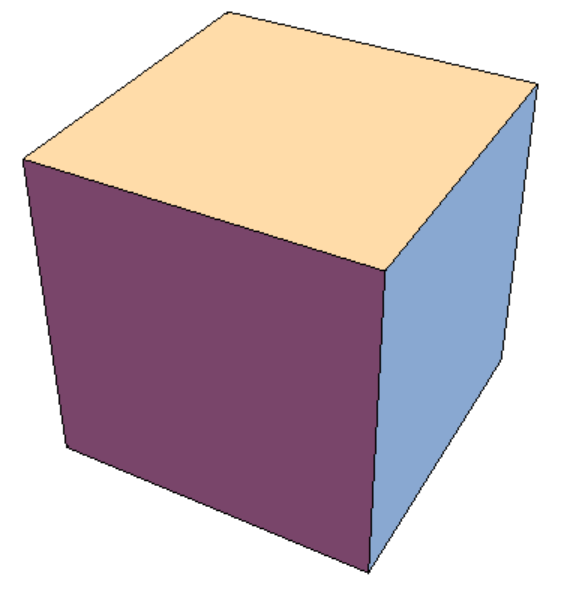
\includegraphics[width=0.3\textwidth]{figures/cube}
	\caption{A figure caption beneath the figure for description of the depicted concept which sometimes can be very long}
	\label{ft_fig_firstfig}
\end{figure}

In \autoref{ft_fig_firstfig}, for example, a PNG image is depicted (compiled with pdflatex). Alternatively, EPS figures can be embedded if dvips and ps2pdf compilation is used. All figures are listed in the list of figures with the command \imp{listoffigures}.

%%%%%%%%%%%%%%%%%%%%%%%%%%%%%%%%%%%%%%%%%%%%%%%%%%%%%%%%%%%
%%%%%%%%%%%%%%%%%%%%%%%%%%%%%%%%%%%%%%%%%%%%%%%%%%%%%%%%%%%

\section{Tables}

Data can be presented in tables, e.g., as shown in \autoref{ft_tab_ex}.

\begin{table}[!h]
	\centering
	\begin{tabular}{l|cl}
	\hline \hline
	
		& Property 1
		& Property 2\\ \hline
	Criterion 1
		& 764
		& 23546 \\
	Criterion 2
		& 3
		& 34 \\
	\hline \hline
	\end{tabular}
	\caption{Exemplary table}
	\label{ft_tab_ex}
\end{table}

Sometimes very long tables must be presented which may also go over pages. For this cases the packages \imp{longtable} is useful, as used in 

\begin{center}
\begin{longtable}{l|l|l}

% \baselinestretch{1.5}

 \hline \hline
 $i^3$ & $2i^3$ & $3i^3$ \bigstrut \\ \hline
 \endfirsthead
 
 \multicolumn{3}{c}{\tablename\ \thetable{} -- information message on top} \\
 \hline
 $i^3$ & $2i^3$ & $3i^3$ \bigstrut \\ \hline 
 \endhead
 
 \hline
 \multicolumn{3}{c}{Foot information} \\ \hline
 \endfoot
 
 \hline \hline
 \caption{Long Table}
 \label{lt}
 \endlastfoot
 
 1 & 2 & 3 \\
 8 & 16 & 24 \\
 27 & 54 & 81 \\
 64 & 128 & 192 \\
 125 & 250 & 375 \\
 216 & 432 & 648 \\
 343 & 686 & 1029 \\
 512 & 1024 & 1536 \\
 729 & 1458 & 2187 \\
 1000 & 2000 & 3000 \\
 1331 & 2662 & 3993 \\
 1728 & 3456 & 5184 \\
 2197 & 4394 & 6591 \\
 2744 & 5488 & 8232 \\
 3375 & 6750 & 10125 \\
 4096 & 8192 & 12288 \\
 4913 & 9826 & 14739 \\
 5832 & 11664 & 17496 \\
 6859 & 13718 & 20577 \\
 8000 & 16000 & 24000 \\
 9261 & 18522 & 27783 \\
 10648 & 21296 & 31944 \\
 12167 & 24334 & 36501 \\
 13824 & 27648 & 41472 \\
 15625 & 31250 & 46875 \\
 17576 & 35152 & 52728 \\
 19683 & 39366 & 59049 \\
 21952 & 43904 & 65856 \\
 24389 & 48778 & 73167 \\
 27000 & 54000 & 81000 \\
 29791 & 59582 & 89373 \\
 32768 & 65536 & 98304 \\
 35937 & 71874 & 107811 \\
 39304 & 78608 & 117912 \\
 42875 & 85750 & 128625 \\
 46656 & 93312 & 139968 \\
 50653 & 101306 & 151959 \\
 54872 & 109744 & 164616 \\
 59319 & 118638 & 177957 \\
 64000 & 128000 & 192000 \\
 68921 & 137842 & 206763 \\
 74088 & 148176 & 222264 \\
 79507 & 159014 & 238521 \\
 85184 & 170368 & 255552 \\
 91125 & 182250 & 273375 \\
 97336 & 194672 & 292008 \\
 103823 & 207646 & 311469 \\
 110592 & 221184 & 331776 \\
 117649 & 235298 & 352947 \\
 125000 & 250000 & 375000 \\
\end{longtable}
\end{center}

All tables are listed with \imp{listoftables}.

%%%%%%%%%%%%%%%%%%%%%%%%%%%%%%%%%%%%%%%%%%%%%%%%%%%%%%%%%%%
%%%%%%%%%%%%%%%%%%%%%%%%%%%%%%%%%%%%%%%%%%%%%%%%%%%%%%%%%%%

\section{Enumerate and itemize}

If important sequential points are to presented the environment \imp{enumerate} can be used as follows:
\begin{enumerate}
\item
	Some important stuff
\item
	More stuff
\end{enumerate}
With the package \imp{enumerate} some options can be used, e.g.,
\begin{enumerate}[a)]
\item
	Some important stuff
\item
	More stuff
\end{enumerate}
or 
\begin{enumerate}[~~~1)]
\item
	Some important stuff
\item
	More stuff
\end{enumerate}

Alternatively, point can be just presented without any enumeration with the environment \imp{itemize}
\begin{itemize}
\item
	Some important stuff
\item
	More stuff
\end{itemize}

%%%%%%%%%%%%%%%%%%%%%%%%%%%%%%%%%%%%%%%%%%%%%%%%%%%%%%%%%%%
%%%%%%%%%%%%%%%%%%%%%%%%%%%%%%%%%%%%%%%%%%%%%%%%%%%%%%%%%%%
%%%%%%%%%%%%%%%%%%%%%%%%%%%%%%%%%%%%%%%%%%%%%%%%%%%%%%%%%%%

\chapter{Appendix, footnotes, todos and index}

%%%%%%%%%%%%%%%%%%%%%%%%%%%%%%%%%%%%%%%%%%%%%%%%%%%%%%%%%%%
%%%%%%%%%%%%%%%%%%%%%%%%%%%%%%%%%%%%%%%%%%%%%%%%%%%%%%%%%%%

\section{Appendix}

For many reasons some concept may be important for the document but too long for the main text. In this kind of cases these concept can be presented with the environment \imp{appendix} in appendices, e.g., as in \autoref{app_ex1} and \autoref{app_ex2}.

%%%%%%%%%%%%%%%%%%%%%%%%%%%%%%%%%%%%%%%%%%%%%%%%%%%%%%%%%%%
%%%%%%%%%%%%%%%%%%%%%%%%%%%%%%%%%%%%%%%%%%%%%%%%%%%%%%%%%%%

\section{Footnotes}

You may want to give additional information to some points\footnote{Bla bla} in the text\footnote{Blu blup}.

%%%%%%%%%%%%%%%%%%%%%%%%%%%%%%%%%%%%%%%%%%%%%%%%%%%%%%%%%%%
%%%%%%%%%%%%%%%%%%%%%%%%%%%%%%%%%%%%%%%%%%%%%%%%%%%%%%%%%%%

\section{Todos}

With the package \imp{todonotes} comments\todo{like this one}\ pointing to their place can be embedded into the text. These comments are veeeery useful if you are writing something for the first time or are working on a draft. The todos can be listed with \imp{listoftodos} where you want it to appear in order to see what is unfinished or needs some more work.

%%%%%%%%%%%%%%%%%%%%%%%%%%%%%%%%%%%%%%%%%%%%%%%%%%%%%%%%%%%
%%%%%%%%%%%%%%%%%%%%%%%%%%%%%%%%%%%%%%%%%%%%%%%%%%%%%%%%%%%

\section{Index}

If the document is very long, it may be very useful for a lot of readers to have an index for searching key words and certain concepts (Crtl+F is usually very helpful in PDFs but not always the best solution). For this, the  package \imp{makeidx}, the commands \imp{makeindex} and \imp{printindex} and the compiling option \imp{make index} are needed. You may want to index different words like heterogeneous materials\index{Heterogeneous materials}, effective properties\index{Effective properties} and homogenization\index{Homogenization}.

%%%%%%%%%%%%%%%%%%%%%%%%%%%%%%%%%%%%%%%%%%%%%%%%%%%%%%%%%%%
%%%%%%%%%%%%%%%%%%%%%%%%%%%%%%%%%%%%%%%%%%%%%%%%%%%%%%%%%%%
%%%%%%%%%%%%%%%%%%%%%%%%%%%%%%%%%%%%%%%%%%%%%%%%%%%%%%%%%%%

\begin{appendix}

%%%%%%%%%%%%%%%%%%%%%%%%%%%%%%%%%%%%%%%%%%%%%%%%%%%%%%%%%%%
%%%%%%%%%%%%%%%%%%%%%%%%%%%%%%%%%%%%%%%%%%%%%%%%%%%%%%%%%%%

\chapter{Just an example appendix}
\label{app_ex1}

%%%%%%%%%%%%%%%%%%%%%%%%%%%%%%%%%%%%%%%%%%%%%%%%%%%%%%%%%%%

\section{Bla blup}

Sme stuff
\begin{equation}
	f(x) = \int_{\Omega} g(x) dx \ .
\end{equation}

%%%%%%%%%%%%%%%%%%%%%%%%%%%%%%%%%%%%%%%%%%%%%%%%%%%%%%%%%%%\\
%%%%%%%%%%%%%%%%%%%%%%%%%%%%%%%%%%%%%%%%%%%%%%%%%%%%%%%%%%%

\chapter{Another example}
\label{app_ex2}

%%%%%%%%%%%%%%%%%%%%%%%%%%%%%%%%%%%%%%%%%%%%%%%%%%%%%%%%%%%

\section{More stuff}

Bla bla.

\end{appendix}

%%%%%%%%%%%%%%%%%%%%%%%%%%%%%%%%%%%%%%%%%%%%%%%%%%%%%%%%%%%
%%%%%%%%%%%%%%%%%%%%%%%%%%%%%%%%%%%%%%%%%%%%%%%%%%%%%%%%%%%
%%%%%%%%%%%%%%%%%%%%%%%%%%%%%%%%%%%%%%%%%%%%%%%%%%%%%%%%%%%

%\bibliographystyle{plain}
\bibliographystyle{abbrvnat}
\bibliography{literature/library}

\listoffigures
\listoftables

\printindex

%%%%%%%%%%%%%%%%%%%%%%%%%%%%%%%%%%%%%%%%%%%%%%%%%%%%%%%%%%%
%%%%%%%%%%%%%%%%%%%%%%%%%%%%%%%%%%%%%%%%%%%%%%%%%%%%%%%%%%%
%%%%%%%%%%%%%%%%%%%%%%%%%%%%%%%%%%%%%%%%%%%%%%%%%%%%%%%%%%%

\end{document}

%%%%%%%%%%%%%%%%%%%%%%%%%%%%%%%%%%%%%%%%%%%%%%%%%%%%%%%%%%%
